\documentclass[letterpaper, 12pt]{article}
\usepackage[letterpaper, top=2.5cm, bottom=2.5cm, left=3cm, right=3cm]{geometry} %margenes
\usepackage[backend=biber]{biblatex}\addbibresource{referencias.bib}
\usepackage[utf8]{inputenc} %manejo de caracteres especiales
\usepackage[spanish]{babel} %manejo de encabezados de inglés a español
\usepackage{fancyhdr} %formato de los encabezados de página
\usepackage{ragged2e} %alineado real justficado
\usepackage{graphicx} %manejo de imagenes
\usepackage{amsmath} %manejo de notación matemática
\usepackage{mathtools} %manejo de notación matemática
\usepackage{blindtext} %texto de relleno
\usepackage{tikz} %manejo de diagramas electricos
\usepackage{circuitikz} %manejo de diagramas electricos
\usepackage{csquotes}
\usepackage[titles]{tocloft} %manejo de elementos para el índice
\usepackage{float} %manejo de centrado para figuras

\pagestyle{fancy}
\fancyhf{}
\rfoot{\thepage}

\nocite{*}

\begin{document}
    
    %PORTADA
    \begin{titlepage}
        \begin{figure}[ht]
            \centering
            
\includegraphics[width=15cm]{logosITT.png}
        \end{figure}
        \centering
        {\scshape\LARGE Tecnológico Nacional de México\\Instituto Tecnológico de Tijuana\par}
        \vspace{1cm}
        {\scshape\Large Princípios Electricos y Aplicaciones Digitales\par}
        \vspace{1cm}
        {\scshape\Large Unidad 1\par}
        \vspace{1.5cm}
        {\huge\bfseries Tarea 1\par}
        \vspace{2cm}
        {\Large\itshape Equipo D1N4Mic B00M\par}
        \vfill
        Profesor: \par
        Ing. Rigoberto Alvarado Rivera
        
        \vfill

        {\large 16 de octubre del 2020}
    \end{titlepage}

    \newpage
    \thispagestyle{empty}
    \tableofcontents
    \listoffigures

    \newpage
    \begin{justify}
        \setcounter{page}{1}
        \thispagestyle{fancy}
        \lhead{\textbf{Tarea 1}}
        \rhead{\text{16 de octubre del 2020}}
        \section{Medición Industrial de corriente}
        \justify
        El ejemplo mas claro y preciso que se explica es el de la marca \emph{HARTING Technology Group} la cual se aprecia en la Figura \ref{fig:MedHalt}.
        \begin{figure}[H]
            \centering
            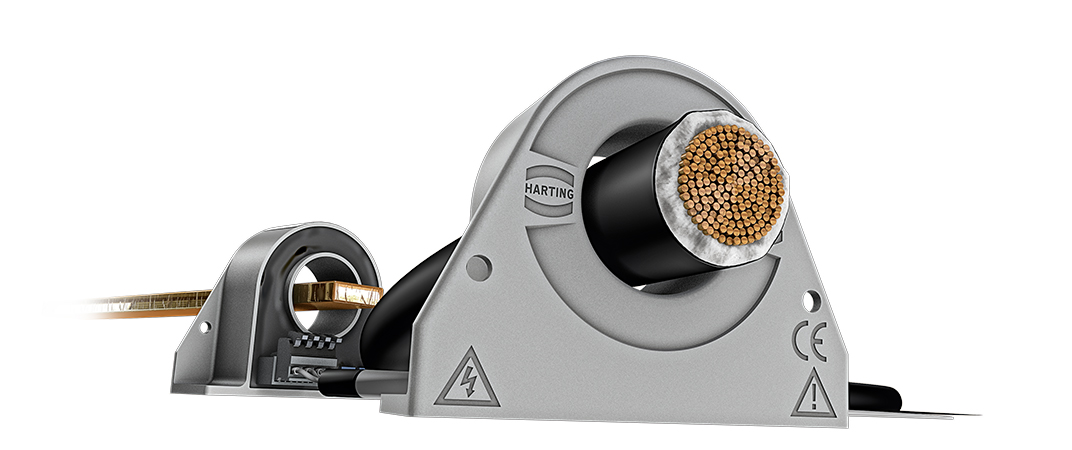
\includegraphics[width=8cm]{HARTING.jpg}
            \caption{Medidor industrial de corriente de \emph{HARTING Technology Group}.}
            \label{fig:MedHalt}
        \end{figure}
        \justify
        Estos sensores son componentes electromecánicos los cuales muestran una representación precisa y en tiempo real de la entrada y la salida de las corrientes.
        Dichas señales son usadas depsues para controlar precisamente a los semiconductores potentes y para monitorear su rendimiento y funcionalidad. Los de la compañia HARTING
        estan basados en el llamado \emph{Efecto Hall}.
        \subsection{Efecto Hall}
        \justify
        De manera breve, este efecto permite medir el voltaje transversal en un conductor cuando es puesto en un campo magnético. Mas allá, aparece una separación de cargas que da lugar a un campo
        eléctrico en el interior del conductor perpendicular al movimiento de las cargas y al campo magnético aplicado, lo cual se puede apreciar en la Figura \ref{fig:Hall}.\\ \newline
        En 1879, Edwin Albert Hall descubrió el efecto que lleva su nombre. Encontró que si se aplica un campo magnético elevado a una fina lámina de oro por la que circula corriente, se produce un voltaje en
        la lámina transversalmente a como fluye la corriente. Con ello podemos medir la intensidad de las corrientes eléctricas.
        \begin{figure}[H]
            \centering
            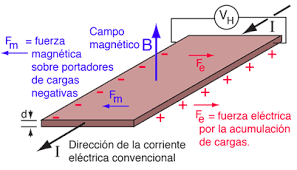
\includegraphics[width=10cm]{Hall.png}
            \caption{Modelo del Efecto Hall.}
            \label{fig:Hall}
        \end{figure}
        \section{La ``Maquina de toques''}
        \justify
        En esencia, el dispositvo eléctrico de bromas por excelencia. Dependiendo de la capacidad de cada uno de sus componentes, dependera su potencia, en este caso se usará
        el mas simple:

        \begin{figure}[ht]
        \centering
        \begin{circuitikz}
        \draw
        (0,0) to[battery] (0,4)
              to[resistor] (4,4) -- (8,4)
        (4,4) to[pC] (4,0) -- (0,0)
        (4,4) to[push button] (8,4)              
        (8,4) node[transformer core,anchor=A1](T){};
        \draw (T.A2) -- (8,0) -- (4,0);
        \end{circuitikz}
        \caption{Circuito sin valores de la maquina de toques.}
        \label{fig:Toques}
        \end{figure}
        \justify
        \subsection{Componentes}
        \begin{itemize}
            \item \emph{Transformador con nucleo de hierro:}  Convierte energía eléctrica AC con cierta tensión a otra energía eléctrica AC con distinta tensión. 
            \item \emph{Interruptor NA (normalmente abiertos):} Parte de los circuitos de conmutación. Este permite el flujo de corriente mientras no se actue sobre ellos.
            \item \emph{Capacitor polarizado:} Usado principalmente como amortiguador de la energía eléctrica; suministra energía cuando se necesite si su corriente es AC y suaviza la misma si ésta es DC.
            \item \emph{Fuente de voltaje:} Coloquialmente conocido como la pila, esta brinda la energía electrica al circuito en forma de voltaje.
            \item \emph{Resistencia:} Permite la reducción de la energía electrica en el circuito para que este no haga corto circuito.
        \end{itemize}
        \subsection{Funcionamiento}
        \justify
        De manera básica y en base al circuito de la Figura \ref{fig:Toques}, este artefacto es un inversor de voltaje. A partir de una pila, un oscilador eléctronico y un transformador de voltaje instalado a la inversa que eleva el voltaje de la pila con un
        mínimo de corriente. \\ \newline
        Como el cuerpo humano está compuesto en gran parte de agua y electrolitos, y estos funcionan como un conductor débil a la electricidad generada por dicho artefacto, el cuerpo siente el flujo eléctrico como
        una descarga eléctrica y debido a que los músculos se contraen por los impulsos nerviosos (los cuales son electricidad), el individuo experimenta dicha reacción sin importar la cantidad de control que se tiene con sus extremidades. 
        \subsection{Semenjanzas con el taser}
        \justify
        Para fines de comprensión, el taser con el cual se hará la comparación será con el X26, pistola taser usada por distintas agencias policiacas a travez del mundo, el cual se aprecia con los componentes a detalle en la Figura \ref{fig:X26}. \\
        \begin{figure}[ht]
            \centering
            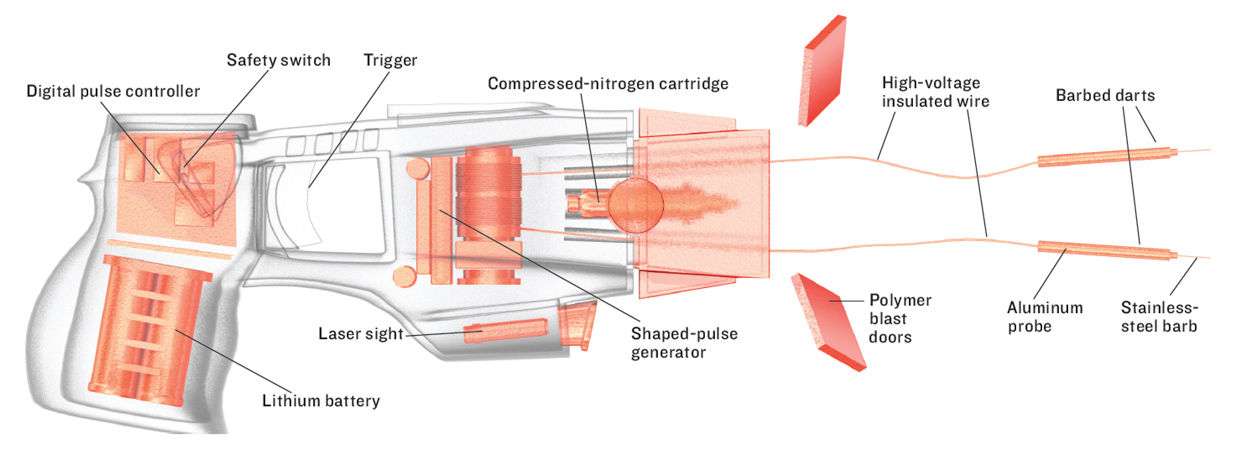
\includegraphics[width=12cm]{tasersqueme.jpeg}
            \caption{Esquema comprensivo de los componentes del taser X26}
            \label{fig:X26}
        \end{figure}
        \justify
        Al jalar el gatillo del artefacto, el cartucho del taser se propulsa por un tubo de nitrogeno comprimido que lanza dos dardos puntiagudos de 9mm con cables de hasta 9m que penetra la ropa y la capa protectora externa de la pila, formando
        la conexión electrica para la descarga. La contracción muscular caraterística causada por este es debido a que los 50 k\(V\) que incialmente se producen se reducen a 1.2 k\(V\) y el circuito genera una serie de 19ppm con una corriente de 1.9 m\(A\),
        cantidades suficientes para la contracción incapacitante del objetivo en cuestión (en este caso, si el disparo acertó al torso como se ilustra en la Figura \ref{fig:effectx26}).
        \begin{figure}[H]
            \centering
            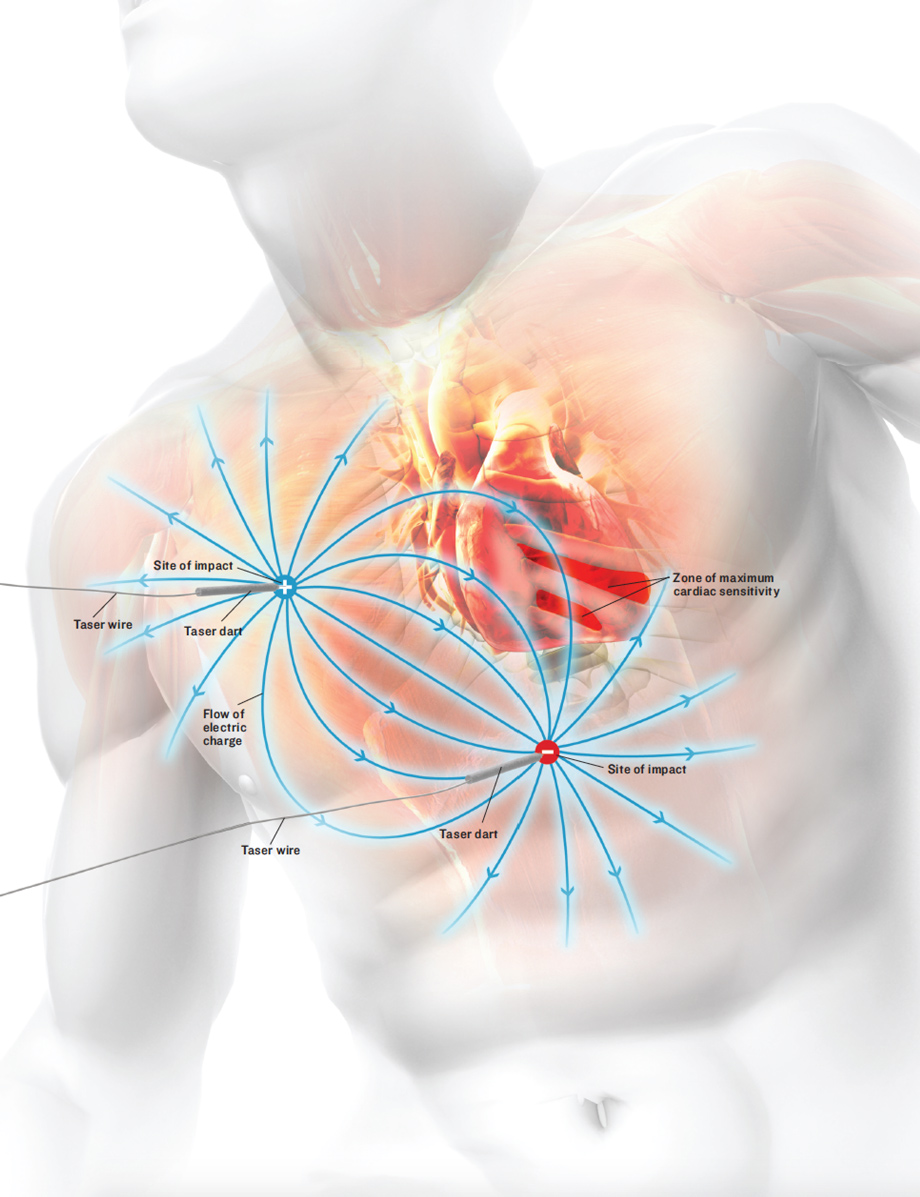
\includegraphics[width=5.2cm]{effectivecont.jpeg}
            \caption{Modelo del efecto incapacitante de un disparo al torso del X26}
            \label{fig:effectx26}
        \end{figure}
        \justify
        Como se explicó en el párrafo anterior, la principal diferencia del taser respecto a la maquina de toques es el mecanismo de funcionamiento el cuál, la maquina de toques es mas simple que el taser X26. Otra difrencia es que el taser se enfoca en dar una serie de ciclos de corriente indicados para
        solamente incapacitar al objetivo, en contraste con la maquina de toques, la cual (se supone) que la exposición a la corriente es voluntaria.
        \section{Ruido generado por los transformadores}
        \justify
        El zumbido caracteristico de los transformadores es generado en el núcleo derivado por la magnetosustitución, y por la laminas cuando el campo magnetico pasa a travez de ellos. Dicho ruido depende de la cantidad de carga que pasa a travez del dispositivo.
        \\ \newline
        Si los ruidos generados por el transformador aumentan la frecuencia, es decir, que es más fuerte, es una indicación de que el transformador tiene algún problema. Esto es porque los componentes son vibroacústicos (generan ruido con la vibración) y si llegaran a
        soltar o sobrecargar los mismos, aumentan la intensidad del zumbido.
        \section{Uso de transformadores en los postes}
        \justify
        Como ya se mencionó brevemente en el punto anterior, los tranformadores transforman (valga la redundancia) la corriente para convertirla en valores mas bajos y que la misma (generalmente 120 a 240 voltios) proporcione la energía suficiente para la gran mayoria de electrodomésticos sin llegar a sobrecargarlos y/o
        averiarlos. 
        \begin{figure}[ht]
            \centering
            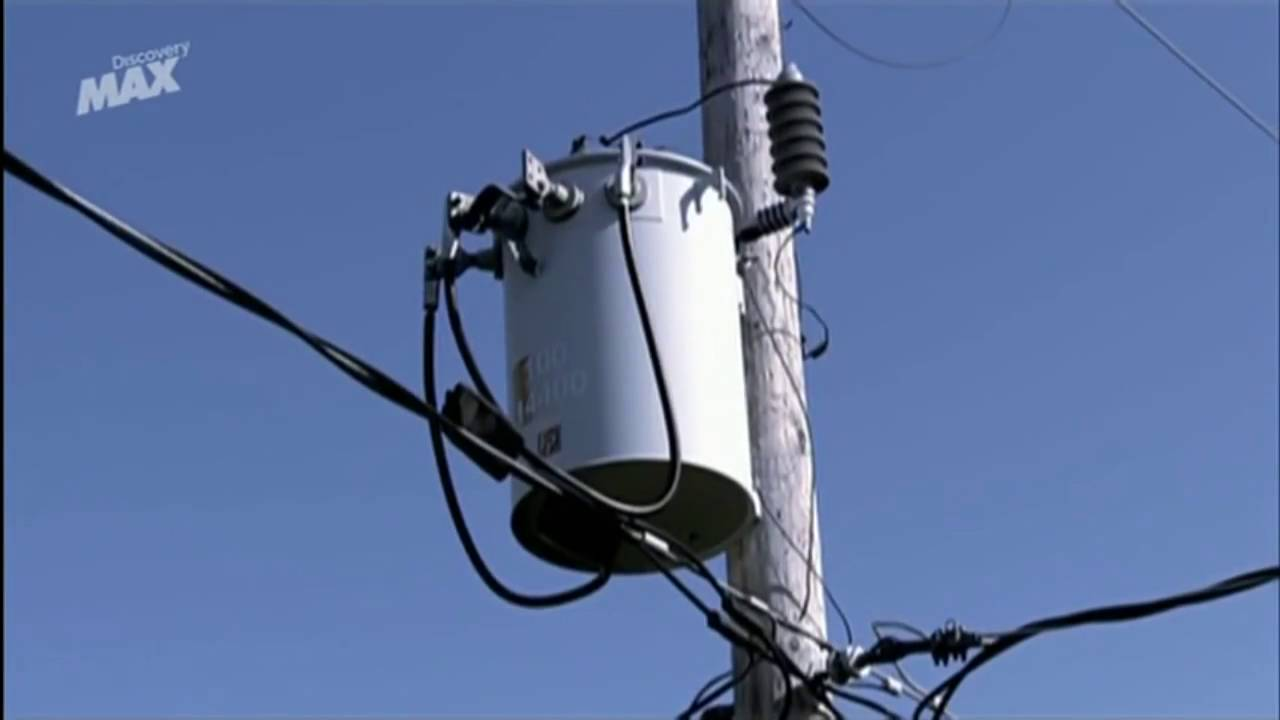
\includegraphics[width=8cm]{trans.jpg}
            \caption{Imágen de un transformador en un poste de luz.}
        \end{figure}        
        \section{Uso de tres cables en los postes de luz}
        \justify
        Como se explico el primer día de clase, la razón por la cual los postes de luz contienen tres cables es debido a que en las plantas de producción de energía eléctrica, estas producen una cantidad bastante grande de voltaje la cual se transporta de mejor manera en un sistema trifásico, la cual aumentan aún mas para que sea transmitida
        a travez de las torres de transmisión fuera de la ciudad. Debido a que continen un voltaje muy alto, se vuelven a convertir en voltajes menos peligrosos para que ahora si sean transmitidos a los reconocibles postes de luz. En la Figura \ref{fig:grid} se puede apreciar con mayor detalle.
        \\ 
        \newline
        Dependiedo del uso esperado para la corriente, estos tres cables pueden:
        \begin{itemize}
            \item Pasar a una corriente trifásica para proveer energía a maquinarias de manufactura debido a que requieren mayor potencia, y por ende mayor energía.
            \item Atenuar la corriente con un transformador residencial, para proveer el voltaje necesario para los electrodomésticos del hogar.
        \end{itemize}
        \begin{figure}[ht]
            \centering
            \label{fig:grid}
            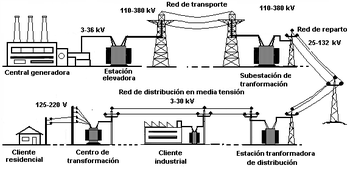
\includegraphics[width=10cm]{themgrid.png}
            \caption{Esquema comprensivo de la red eléctrica desde su generación hasta su distribución doméstica.}
        \end{figure}
        \section{Cargadores inalámbricos}
        \justify
        Una de las alternativas de carga para los dispositivos móviles es la de los cargadores inalámbricos.\\
        \begin{figure}[H]
            \centering
            \label{fig:wireless}
            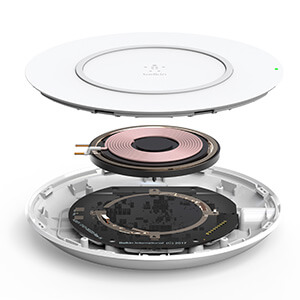
\includegraphics[width=6cm]{wireless.jpg}
            \caption{Componentes básicos de un cargador inalámbrico. El mas destacable es la bobina de cobre.}
        \end{figure}
        \subsection{Funcionamiento}
        \justify
        De manera mas específica, la carga inalámbrica es realmente una carga por inducción (carga electromagnética) lo cual es evidente debido a la Figura \ref{fig:wireless}. Dicho sistema es bastante sencillo en lo a su ejecución respecta.
        \\ Consiste en generar un campo electromagnético y emisor de energía, y lograr captar la energía en el otro extremo. Dicho campo es el soporte para el celular y el receptor es el teléfono.
        \subsection{Ventajas y desventajas en contraste con un cargador alámbrico}
        \subsubsection{Ventajas}
        \begin{itemize}
            \item Comodidad para cargar el aparato.
            \item No hay algún tipo de desgaste de medio de conexión debido a que es sin cable.
            \item Debido a que distintos cargadores inalámbricos mantienen el estandar Qi, los mismos dispositivos son de entrada ``universal''.
        \end{itemize}
        \subsubsection{Desventajas}
        \begin{itemize}
            \item El mayor incoveniente es que, de manera irónica se necesita un cable para conectar la plataforma de carga a la red eléctrica.
            \item Continuando el incoveniente de la plataforma de carga, se necesita forzosamente mantener el dispositivo sobre la plataforma para el flujo eléctrico.
            \item Las velocidades de carga entre los dispositivos inalámbricos no son consistentes. Así que por las limitaciones tecnológicas la carga alámbrica sigue siendo muy superior.
        \end{itemize}
    \end{justify}
     
    \newpage
    \addcontentsline{toc}{section}{Referencias}
    \printbibliography

\end{document}